\section{Methodology}
\label{sec:methodology}


This section presents the design and implementation of \tool. We begin by providing a high-level overview of the framework's architecture (Section~\ref{sec:overview}). We then detail the core stages of our simplification pipeline: the variable normalization process that canonicalizes input formulas (Section~\ref{sec:normalization}), the feature encoding and predictive model training that constructs the agent's state representation (Section~\ref{sec:feature-encoding}), the multi-level hybrid reward system (Section~\ref{sec:reward-system}), and our dual-agent policy formulation that synergizes \RL{} and \LLM{}s (Section~\ref{sec:policy-formulation-and-optimization}). Finally, we detail the simplification algorithm (Section~\ref{sec:algorithm}).

For clarity of terminology, we use ``semantics-aware'' to denote the policy-learning paradigm and reasoning that leverages program semantics during variable-level concretization, and ``semantics-guided'' to denote the \LLM{}-driven value proposal subroutine whose candidate values are guided by semantic cues.
\wyc{Overall comment: I think lots of contents are generated by llm. you should write your on own. LLMs are only used for polishing.}

% This section details the design of \tool.
% In this section, we present our methodology, in particular, we discuss the major components including deoptimization, performance checking and test case reduction in detail.

% This section presents the technical blueprint \wyc{uncommon to use `blueprint', refer to existing paper.} for \tool, our AI-assisted framework that reframes the challenge of \SMT{} constraint simplification as a policy-learning problem. Building upon the intuition from Section~\ref{sec:motivating-example} and the formalization in Section~\ref{sec:problem-formalization}, we operationalize our vision of an intelligent agent that learns expert-like simplification strategies. The core of our methodology is a synergistic framework where a \RL{} agent learns the high-level policy of what to simplify (\ie, selecting the most impactful variable), while a \LLM{} provides the semantic intuition for how to simplify it (\ie, generating a promising concrete value).

\wyc{The content before sec 4.1 is too long, usually we only illustrate what this section do, \eg, ``In this section, we present our methodology, in particular,
we discuss the major components including deoptimization,
performance checking and test case reduction in detail.''

However, the last paragraph (start with "for clarity..." is ok.)
}
\subsection{Overview}
\label{sec:overview}


\begin{figure}[t]

    \centering
    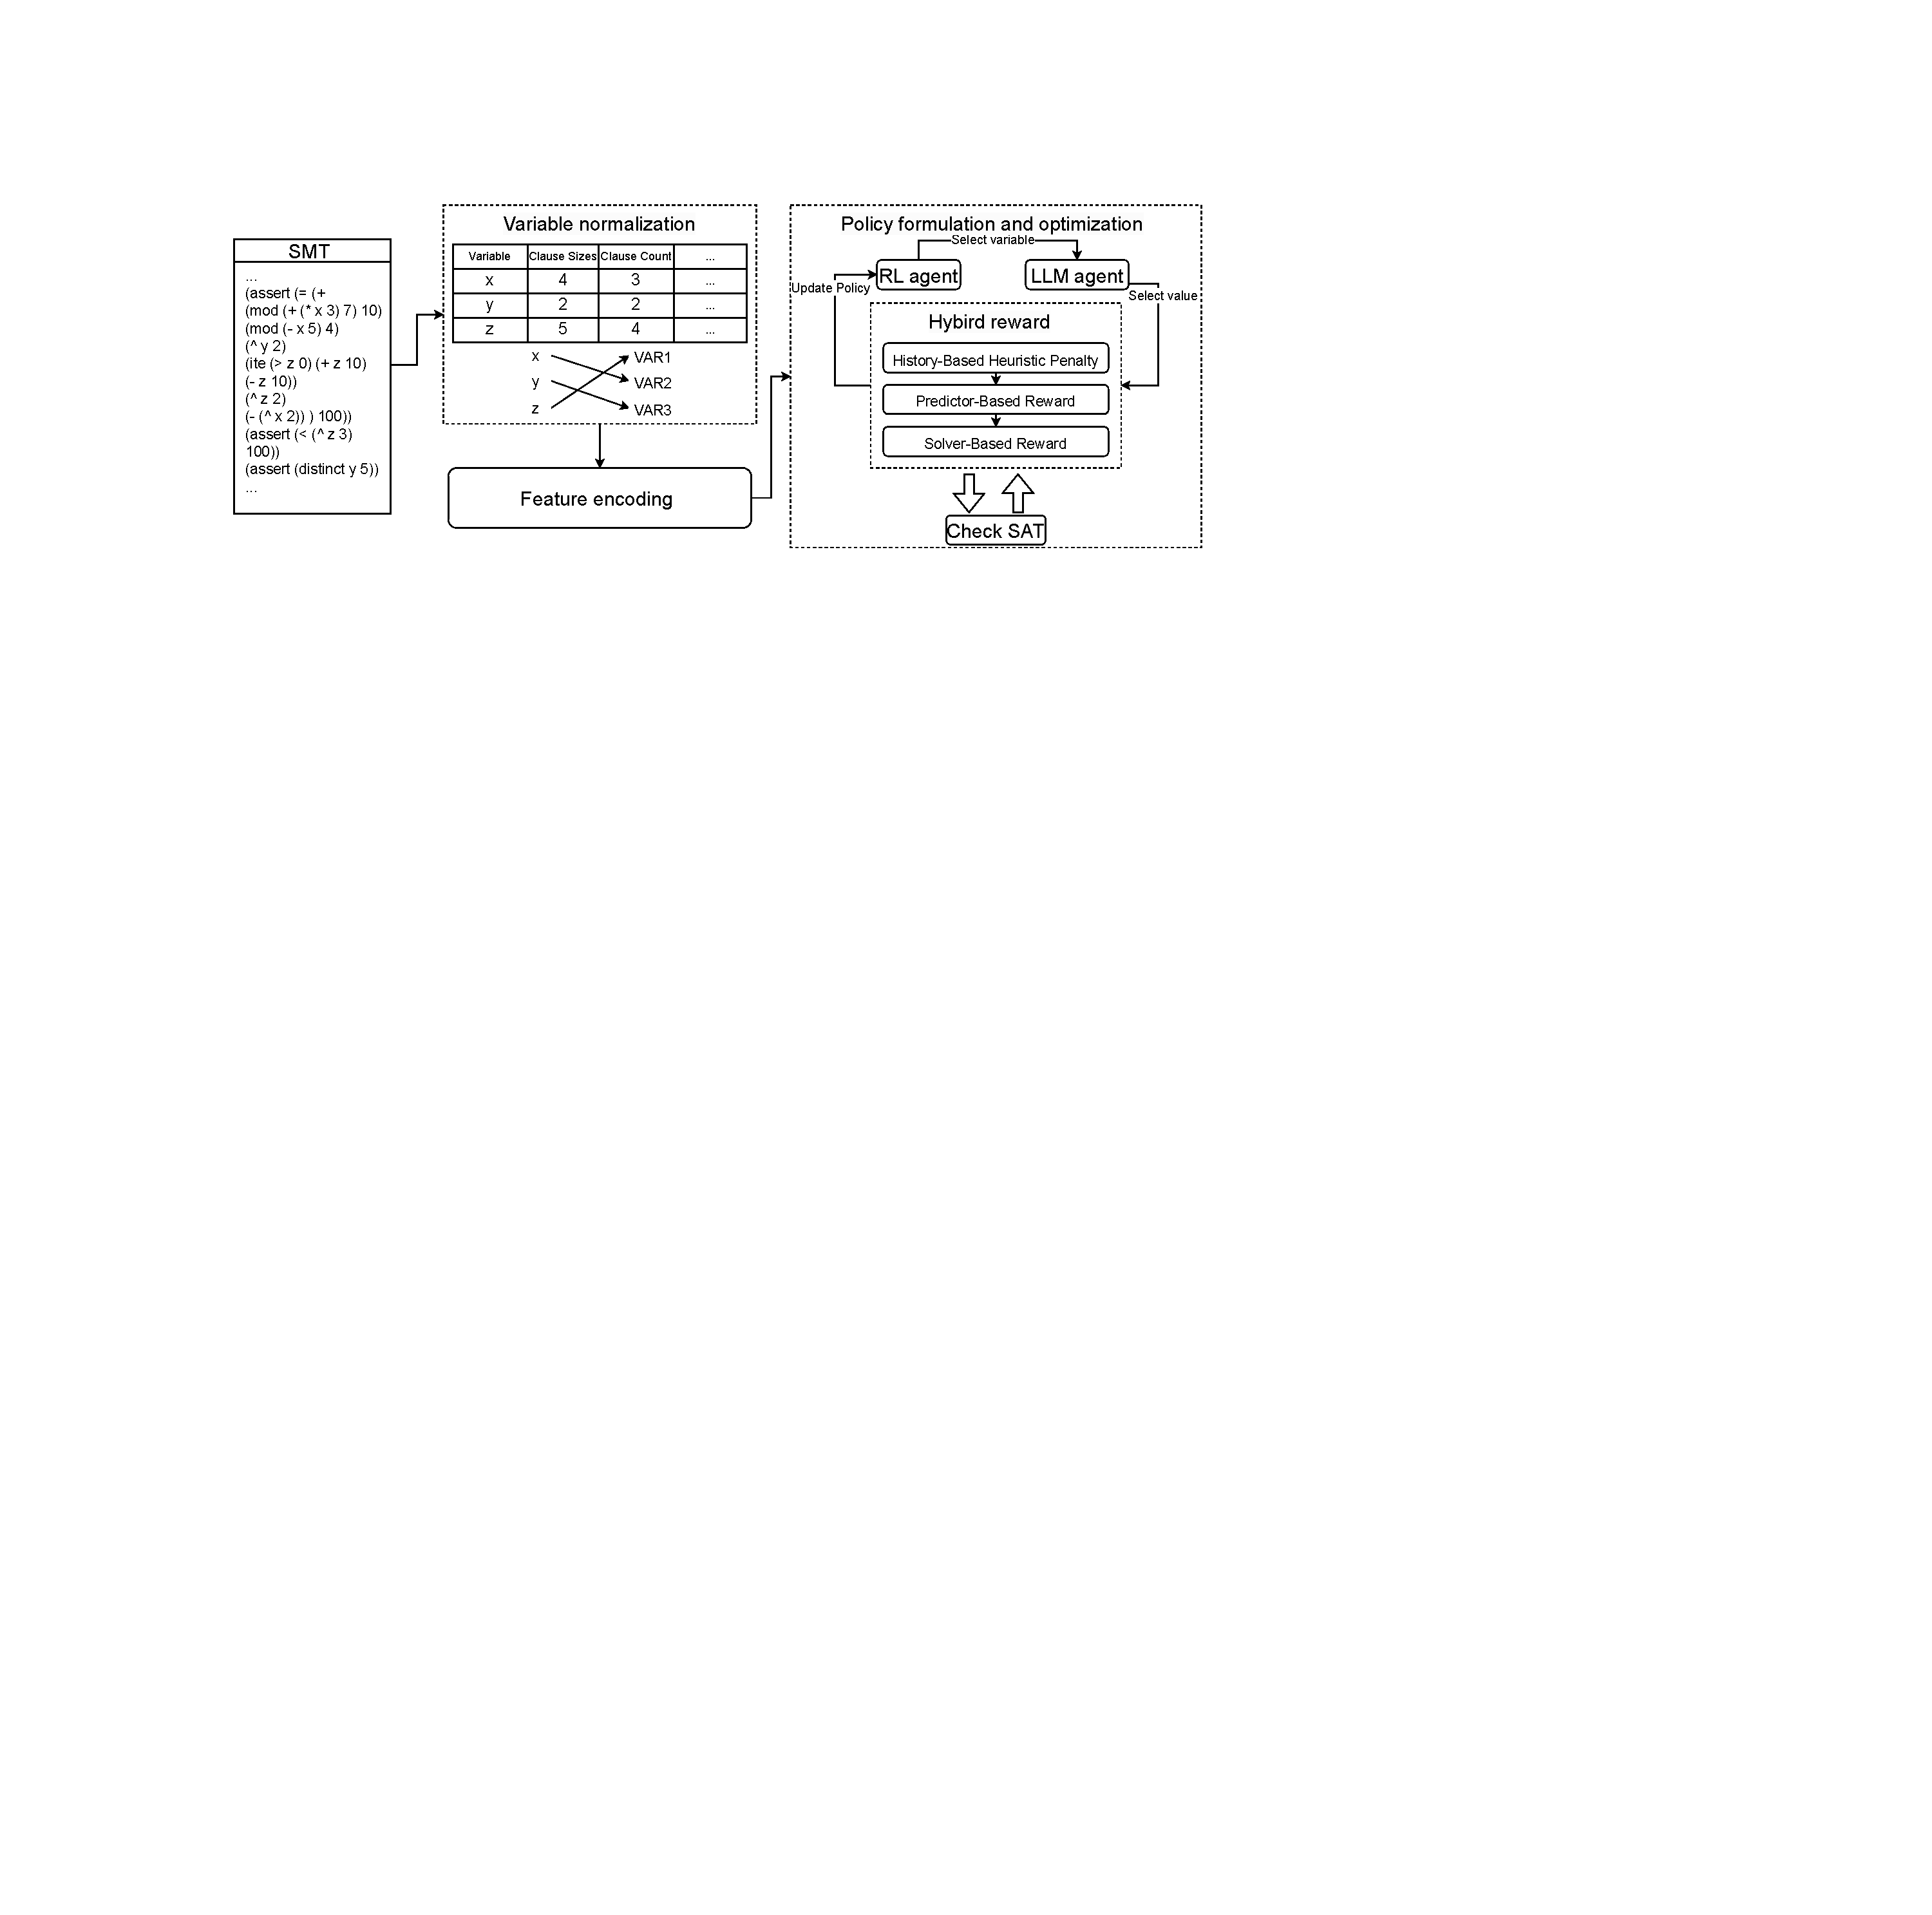
\includegraphics[width=\linewidth]{pics/method.pdf}
    \caption{Workflow of \tool{}.}
    \label{fig:method}
\end{figure}

Figure~\ref{fig:method} illustrates the architecture of \tool{}， which consists of four components: variable normalization, feature encoding, hybrid reward system, and dual-agent simplification policy.
% \wyc{use the following: Figure~\ref{fig:method} illustrates the architecture of \tool{}, which consists of xxx components: xxx, xxx, xxx. 
% Then, use what you have written, \ie, The process begins with...} \wyc{The components you introduced must be consistent with that in the workflow.}
The process begins with variable normalization which creates a consistent foundation for learning. To ensure our models can generalize across formulas that are structurally identical but use different variable names, this stage canonicalizes the input by sorting variables based on a stable vector of their structural attributes, yielding a permutation-invariant representation for the agent.

The canonical formula is then transformed into a state representation by our feature encoding component. This component converts the symbolic text into a high-dimensional vector designed to capture the formula's underlying structure. This vector serves two primary purposes. First, it provides the contextual input required for the \RL{} agent's policy decisions. Second, it is used to train two predictive models: a classifier to estimate a formula's solvability and another to predict its solving time.  As we will see, these pre-trained predictors are crucial for guiding the agent's learning.

To guide the learning process effectively, we then designed a hybrid reward system. Recognizing that feedback in the \SMT{} environment is inherently sparse and expensive, this system provides a rich learning signal by combining sparse but definitive outcomes from the \SMT{} solver, dense heuristic guidance from pre-trained predictive models, and history-based penalties to prune the search space.

Finally, guided by this rich reward signal, the heart of our approach is the dual-agent architecture. This architecture is designed to address the challenge of learning over the environment's vast, composite discrete action space, where a complete action consists of both a variable and a value. Instead of learning a single, monolithic policy to navigate this space, our solution decomposes the decision-making process into two complementary roles. A strategic \RL{} agent learns a policy to select what to simplify (variable selection), effectively deciding which dimension of the action space to explore. Subsequently, a tactical \LLM{} uses its semantic reasoning capabilities to propose \textit{how} to simplify (value generation), completing the action pair. This division of labor allows each component to leverage its unique strengths---the RL agent for long-term, feedback-driven planning and the LLM for rich, context-aware reasoning.


\subsection{Variable Normalization}
\label{sec:normalization}
\wyc{This subsection seems not clear to me. The method should be explained more clear (discuss steps first, then explain the benefit.). \eg, adding examples. Second, the design choice is missing (\eg, why do you use the canonicalization method). Finally, why does this method work?}

A foundational challenge for applying machine learning methods to symbolic formulas is input variance~\cite{zaheer2017deep,battaglia2018relational}: two structurally isomorphic formulas may be textually distinct due to arbitrary variable naming, which prevents a learned model from generalizing. To overcome this, \tool{} begins with a deterministic canonicalization of the input SMT formula. The goal of this process is to standardize the naming and ordering of variables based on their structural roles, ensuring that any two structurally equivalent formulas are mapped to the exact same textual representation. This allows our learning models to focus on the underlying semantic structure rather than superficial naming conventions.

\subsubsection{Canonicalization via Structural Sorting}
The core of this process is a deterministic sorting process that reorders variables based on their structural importance. For each variable, we first extract a vector of numerical attributes that serve as proxies for its influence within the formula. These attributes, detailed in Table~\ref{tab:normalization-attributes}, are arranged in a predefined order of importance, including metrics like the total size of clauses a variable appears in, its frequency, and the number of distinct clauses it participates in.
The sorting itself is performed using this ordered vector of attributes. Specifically, all variables are first sorted according to the most important attribute (\ie, `Variable clause sizes'). Any ties among variables are then resolved by sorting them according to the second most important attribute (`Variable to clause count'), and this tie-breaking process continues sequentially down the entire attribute list. This stable, multi-level sorting procedure guarantees that a unique and deterministic ordering is produced for any given formula. Finally, the sorted variables are systematically renamed to a canonical form, such as $\mathit{VAR}_1, \dots, \mathit{VAR}_n$, completing the canonicalization.

\subsubsection{Impact on Policy Learning}
A simpler approach, like alphabetical sorting, would be brittle and fail to capture any structural information. In contrast, our chosen attributes act as robust proxies for a variable's semantic importance, a principle that aligns with feature engineering for code analysis~\cite{henkel2023neural}. By encoding this importance into the variable ordering, we create a representation that is not only consistent but also informative for the downstream agent. This method is effective because it makes the learning models invariant to superficial syntactic differences, a crucial step when applying machine learning to source code~\cite{alon2019code2vec}. This process significantly reduces the variance of the state space the \RL{} agent must explore~\cite{bengio2009learning}, provides a stable action space where an action consistently targets a variable of similar structural importance, greatly simplifying the policy learning challenge~\cite{laskin2021urlb}.
\begin{table}[!t]
    \centering
    \caption{Attributes for variable normalization, ordered by importance.}
    \label{tab:normalization-attributes}
    \begin{tabular}{@{} l p{0.72\linewidth} @{} }
    \toprule
        \multicolumn{1}{c}{\textbf{Attribute}} & \multicolumn{1}{c}{\textbf{Description}} \\ \midrule
        Variable clause sizes   & The sum of elements in clauses where the variable appears. \\ 
        Variable to clause count & The number of distinct clauses the variable appears in. \\ 
        Variable frequencies & The total number of times the variable occurs in the formula. \\ 
        Total logic operations & The number of logical operations the variable participates in. \\ 
        Variable constant interactions & The count of clauses where the variable appears with a constant. \\ \bottomrule
    \end{tabular}
\end{table}
\subsection{Feature Encoding}\lz{introduce "what" in overview, introduce "why" in this section with short explanation}
\label{sec:feature-encoding}
To enable an \RL{} agent to make informed decisions, the \SMT{} formula must be transformed into a rich, machine-readable state representation. It is well-established that purely syntactic representations often fail to capture the complex semantic relationships within structured code or logical formulas, limiting the generalization capabilities of learning models~\cite{alon2019code2vec}. We therefore employ a \PLM{} to serve as our feature encoder, a technique that has proven highly effective for generating deep, contextualized representations of source code~\cite{feng2020codebert}.

% To enable the \RL{} agent to make informed decisions, the SMT formula must be transformed into a machine-readable state representation that captures its underlying semantic properties. While purely syntactic representations often fail to capture such complex relationships and thus limit model generalization~\cite{alon2019code2vec}, pre-trained language models (PLMs) have proven highly effective for generating deep, contextualized representations of structured text like source code~\cite{feng2020codebert}. We therefore employ a PLM-based feature encoder. Unlike handcrafted feature engineering, which would be brittle and difficult to scale across different SMT logics, this approach allows for the automatic learning of semantic nuances directly from data. The entire normalized SMT formula is provided as input to the encoder, which produces a holistic, fixed-size vector embedding to serve as the complete state representation, $s_t$, for the \RL{} agent.


% The encoding process leverages the PLM's ability to comprehend structured text. The entire normalized \SMT{} formula is provided as input to the model, which processes it to produce a holistic, fixed-size vector embedding. This vector is designed to capture the rich semantic relationships and overall structure of the constraints, serving as the complete state representation, $s_t$, for the \RL{} agent at timestep $t$.

% The design rationale behind using a PLM is its ability to learn effective feature hierarchies automatically from data, a core principle of deep learning~\cite{bengio2013representation}. Unlike handcrafted feature engineering, which would be brittle and difficult to scale across different \SMT{} logics, a PLM can automatically learn to capture the semantic nuances of operators, the relationships between variables, and the overall structure of the formula. This method is effective because it provides the \RL{} agent with a dense, semantic state that implicitly encodes much of the information an expert might use for reasoning. A high-quality state representation is fundamental to an agent's ability to learn a non-trivial and generalizable policy, especially in complex domains where such representations can make the learning problem significantly more tractable~\cite{sutton2018reinforcement}.

\subsection{The Hybrid Reward System}
\label{sec:reward-system}

Effective policy learning in \RL{} hinges on receiving frequent and informative feedback. However, the SMT solving environment presents two fundamental challenges for reward design. First, the SMT solver is a well-known performance bottleneck~\cite{cadar2013symbolic}; relying solely on its ground-truth outcomes would require invoking it after every action, rendering the learning process computationally intractable. Second, the environment's rewards are naturally sparse. An agent may perform a long sequence of simplification actions before receiving a definitive outcome, a classic challenge in \RL{} known as the temporal credit assignment problem~\cite{sutton2018reinforcement}.

To overcome these challenges, we designed a hybrid reward system that synergistically combines signals from two distinct real-time sources---the solver and a set of predictive models---and augments them with a history-based heuristic penalty. Crucially, to balance the trade-off between signal density and computational cost, the system employs a partial evaluation strategy, where feedback is periodically generated from a random subset of the formula's constraints rather than the entire set.

\subsubsection{Solver-Based Reward}
The most definitive feedback originates from the SMT solver, providing a high-fidelity, ground-truth signal. The solver's primary role is to provide the ultimate reward through a comprehensive check on the entire formula, typically triggered once at the end of an episode. This anchors the policy to the true objective but is inherently sparse. To enrich the learning process with more frequent feedback, we also employ the solver strategically for partial evaluations. These lightweight checks involve invoking the solver with a short timeout on a subset of constraints, from which a quick \texttt{unsat} result yields a medium-fidelity negative reward, enabling efficient pruning of the search space at a much lower computational cost.

\subsubsection{Predictor-Based Reward}
Complementing the solver, our pre-trained predictive models offer a continuous stream of low-cost, dense guidance. Specifically, we employ two distinct neural network models: a binary classifier, $P_{solve}$, that predicts the likelihood of a formula being satisfiable, and a multi-class classifier, $P_{time}$, that estimates the solving time by assigning it to a predefined complexity bucket.

To ensure the integrity of our evaluation and prevent any data leakage, these predictors are trained on a separate partition of the data. For each benchmark dataset used in our experiments, we perform a strict 50/50 split: one half is used exclusively for training $P_{solve}$ and $P_{time}$, while the other half is reserved as the test set for our online simplification agent. 

During the simplification process, these lightweight models provide the reward signal in two primary ways. They are tightly integrated with our partial evaluation strategy, where they are queried on the same constraint subset as the solver to provide an immediate estimate of progress. Furthermore, their low computational cost allows them to be queried on the full formula at any step, ensuring a constant stream of moment-to-moment feedback. This dense signal directly mitigates the temporal credit assignment problem and provides a smooth learning gradient for the agent.


\subsubsection{History-Based Heuristic Penalty}
In addition to the two real-time reward sources, our system incorporates an orthogonal component that leverages the agent's past experience: a history-based heuristic penalty. This mechanism functions as a form of agent memory, utilizing a repository of counterexamples that stores previously failed action sequences. If the agent's current action sequence matches a known failing path, a significant negative penalty is immediately applied. This low-cost lookup operation acts as an efficient search-space pruning mechanism and provides a deterministic penalty for repeated mistakes, thereby accelerating policy convergence.

\subsubsection{Synergy}
The final reward signal $r_t$ is a synergistic composition of these components. The definitive but sparse signals from full solver evaluations ensure the policy converges towards the true objective. Meanwhile, the combination of denser feedback from partial solver checks and continuous heuristic guidance from the predictors provides a rich gradient for exploration. Finally, the history-based penalty leverages memory to efficiently prune the search space. Together, they form a robust and efficient hybrid reward function capable of guiding the agent through the challenging landscape of SMT constraint simplification.

\subsection{Dual-Agent Architecture}
\label{sec:policy-formulation-and-optimization}

To learn an effective simplification strategy, we formalize the task as a \MDP{} and train a \RL{} agent. The agent's goal is to learn a policy, $\pi(a_t|s_t)$, that maps a given formula state to a simplification action that maximizes the expected long-term reward.
This section details our complete \MDP{} formulation by defining its core components---the state representation ($s_t$), the action space ($a_t$), and the hybrid reward ($r_t$)---and concludes by detailing the approach for optimizing the agent's policy.

\subsubsection{State Representation}
The agent's decision at each timestep is conditioned on the current state of the formula, $s_t$. As defined in Section~\ref{sec:feature-encoding}, we use the high-dimensional vector embedding produced by a \PLM{} as the state representation. This vector captures the rich semantic and structural properties of the canonicalized formula, providing the necessary context for the policy.

\subsubsection{Action Space and Dual-Agent Design}
The action space for simplification is a complex, hybrid domain $\mathcal{A} = \mathcal{V} \times \mathcal{C}$, where $\mathcal{V}$ is the finite, discrete set of canonical variables, and $\mathcal{C}$ is the virtually infinite set of possible integer values. A single RL agent cannot tractably learn a policy over this joint space.
Our core contribution is to decompose this action into two sequential sub-problems, governed by the principle of task decomposition based on the core strengths of each component\cite{kautz2022third}. The high-level, strategic decision of \textit{what} variable to simplify is assigned to an RL agent, whose policy operates over the finite space $\mathcal{V}$. Conversely, the low-level, tactical decision of \textit{how} to simplify is delegated to a pre-trained LLM. Conditioned on the state and the chosen variable, the LLM generates a contextually plausible value. This is achieved by providing it with a carefully constructed prompt that includes the full formula context, the target variable, and a list of previously failed values (counterexamples) to steer it away from known unsuccessful attempts, as shown in Figure~\ref{fig:prompt}. 
A key consequence of this design is that only the RL agent undergoes online, gradient-based policy updates, while the LLM remains a static, pre-trained model with frozen parameters, adapting only through the in-context information provided in the prompt. This paradigm of pairing a dynamic, learning policy with a static, pre-trained model has proven effective for training large models with reinforcement learning. For instance, Ouyang \etal~\cite{ouyang2022training} use a frozen reference model to regularize the policy during optimization, ensuring its core capabilities are preserved. In our framework, the LLM serves as a stable source of general semantic knowledge, while the RL agent specializes in learning a policy for the specific task of SMT simplification.
This is intentional, as it preserves the specialization of each agent. The \RL{} agent's role is to adapt and learn a domain-specific strategy, while the LLM's role is to serve as a stable source of general semantic knowledge. Attempting to fine-tune the LLM on the sparse and noisy reward signal from the solver would risk catastrophically degrading its valuable pre-trained abilities and would be computationally infeasible. While the LLM does not learn via gradients, it does adapt within an episode through in-context learning: by incorporating previously failed values into its prompt as counterexamples, it is steered away from known unpromising suggestions.

\subsubsection{Hybrid Reward}
To guide the agent's learning, we use the multi-level hybrid reward system detailed in Section~\ref{sec:reward-system}. The final reward, $r_t$, for taking a complete action $a_t = (v_t, c_t)$ is a composite signal combining sparse, ground-truth feedback from the solver with dense, estimated rewards from our predictive models. This hybrid reward is crucial for mitigating the credit assignment problem. We emphasize that the LLM is part of the action-generation process, not the reward-generation process.

\subsubsection{Policy Optimization via Soft Actor-Critic}
We learn the variable selection policy $\pi$ using \SAC{}~\cite{haarnoja2018soft}, an off-policy actor-critic method based on the maximum entropy framework. Its selection is principally motivated by two features that directly address the challenges of SMT constraint simplification. First, interacting with the environment is computationally expensive due to the cost of SMT solver invocations. As an off-policy method that leverages a replay buffer, \SAC{} is highly sample-efficient, making it well-suited for learning in environments where data collection is costly~\cite{levine2020offline}. Second, the space of effective simplification strategies is vast and requires extensive exploration to avoid converging to a suboptimal policy. The core mechanism of SAC, entropy maximization, encourages robust exploration by incentivizing the agent to act as randomly as possible while still accomplishing its objective, a critical feature for complex decision-making problems~\cite{haarnoja2018soft}. The \SAC{} agent consists of an actor network, which models the policy, and critic networks, which estimate the expected future rewards. The learning process follows a standard online RL loop. At each step, the agent observes state $s_t$, selects a variable $v_t$, the LLM proposes a value $c_t$, and the environment returns the hybrid reward $r_t$ and the next state $s_{t+1}$. This transition $(s_t, v_t, r_t, s_{t+1})$ is stored in a replay buffer. The agent is then trained by sampling mini-batches from this buffer to update its actor and critic networks, progressively improving its policy to maximize the expected cumulative reward.

\begin{figure}[!t]
    \centering
    \label{fig:prompt}
    \Description{An example of the prompt structure used to query the Large Language Model for value suggestions, including context from the SMT formula.}
    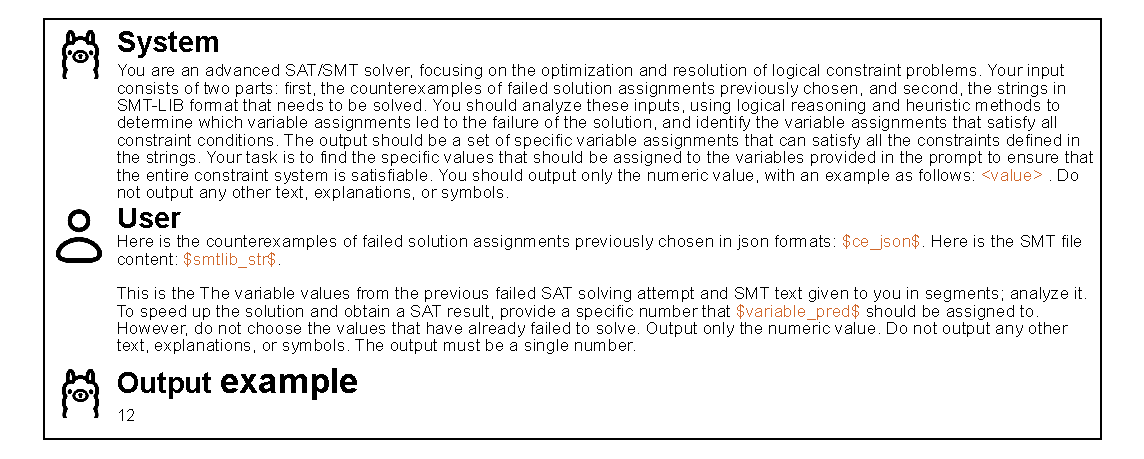
\includegraphics[width=\textwidth,trim=0 8pt 0 8pt,clip]{pics/prompt.pdf}
    \caption{Prompt template for heuristic value generation by the LLM.}
\end{figure}

% \wyc{"Overall Algorithm" seems to be a better title of the subsection}

% \wyc{give the high-level idea of the algorithm (\eg, explain the alg using three major steps), then explain the algorithm line by line.}

% The individual components of our methodology are orchestrated by a single, closed-loop algorithm that operationalizes our framework. As detailed in Algorithm~\ref{alg:main}, this procedure follows a strategic, trial-and-error exploration process, structured as a nested loop. The outer loop initiates new simplification attempts, or "trials," while the inner loop extends the current simplification sequence step-by-step. This process synergistically integrates the components detailed previously: the algorithm is initialized using our variable normalization and feature encoding schemes; the inner loop is driven by the dual-agent policy; and the agent's learning is guided by the multi-level hybrid reward system. A key innovation of this process is a performance-monitoring mechanism that uses our predictive models to greedily extend promising simplification paths, while quickly abandoning and learning from those that degrade performance.

% The algorithm begins by preparing the necessary components for a given formula, $Q_{init}$ (Lines~\ref{alg:line:normalize}--\ref{alg:line:init-history}). This involves applying our variable normalization process (Section~\ref{sec:normalization}) to the initial formula and initializing the SAC agent and the history of counterexamples. The outer loop (Line~\ref{alg:line:outer-loop}) then manages the overall simplification process under a global time budget, initiating new trials as needed.

% Each trial starts by resetting the environment to the original, canonicalized formula, $Q_{base}$ (Line~\ref{alg:line:trial-reset}). The feature encoding component (Section~\ref{sec:feature-encoding}) is invoked to generate the initial state embedding, $s$, and a baseline performance score, $last\_perf$, is initialized to zero (Line~\ref{alg:line:perf-init}). This provides a neutral starting point for performance comparison throughout the trial. The inner loop (Line~\ref{alg:line:inner-loop}) then begins to extend the current simplification sequence. At each step, the dual-agent policy (Section~\ref{sec:policy-formulation-and-optimization}) is executed: the RL agent selects a variable $v_t$, and the LLM proposes a value $c_t$ based on the accumulated counter-examples from previous failed trials (Lines~\ref{alg:line:select-var}--\ref{alg:line:propose-val}).

% After the formula is simplified, the framework evaluates the new state. The feature encoder is re-invoked to produce the next state embedding $s'$ (Line~\ref{alg:line:embed-next}), and the backend solver attempts to solve the modified formula. The multi-level hybrid reward computation simultaneously evaluates both the reward signal and a performance score, $current\_perf$, based on predictive model outputs and solver results (Line~\ref{alg:line:compute-reward}). This performance check is the primary driver of the exploration strategy. If the score degrades compared to the baseline (Line~\ref{alg:line:reset-cond}), the current trial is deemed a failure. The failing sequence is recorded (Line~\ref{alg:line:add-history}), and the inner loop terminates, triggering a new trial. Otherwise, the agent's policy is updated using the full multi-level hybrid reward (Line~\ref{alg:line:compute-reward}), as detailed in Section~\ref{sec:reward-system}, and the state is advanced for the next iteration (Line~\ref{alg:line:advance-state}).

\subsection{Overall Algorithm}
\label{sec:algorithm}
\wyc{"Overall Algorithm" seems to be a better title of the subsection}

\wyc{give the high-level idea of the algorithm (\eg, explain the alg using three major steps), then explain the algorithm line by line.}
The individual components of our methodology are orchestrated by the \tool algorithm, a single, closed-loop procedure that operationalizes our framework, as detailed in Algorithm~\ref{alg:main}. The algorithm follows a strategic, trial-and-error exploration process structured as a nested loop: an outer loop initiates new simplification attempts (``trials''), while an inner loop extends the current simplification sequence step-by-step. A key innovation guiding this process is a performance-monitoring mechanism that defines the ``error'' phase of this exploration: it uses our predictive models to greedily pursue promising paths while quickly abandoning those that degrade performance. These abandoned sequences are treated as learning opportunities---``errors''---and are recorded as counterexamples to inform subsequent trials. The process begins by preparing the initial formula $Q_{init}$ through variable normalization and initializing the \SAC{} agent and the repository for these counterexamples (Lines~\ref{alg:line:normalize}--\ref{alg:line:init-history}). The outer loop then manages the overall simplification process, launching new trials until a satisfying assignment is found or an external termination condition (\eg, a timeout) is met (Line~\ref{alg:line:outer-loop}).

Each trial starts by resetting the environment to the original, canonicalized formula, $Q_{base}$ (Line~\ref{alg:line:trial-reset}). The feature encoding component (Section~\ref{sec:feature-encoding}) is invoked to generate the initial state embedding, $s$, and a baseline performance score, $last\_perf$, is initialized to zero (Line~\ref{alg:line:perf-init}). This provides a neutral starting point for performance comparison throughout the trial. The inner loop (Line~\ref{alg:line:inner-loop}) then begins to extend the current simplification sequence. At each step, the dual-agent policy (Section~\ref{sec:policy-formulation-and-optimization}) is executed: the RL agent selects a variable $v_t$, and the LLM proposes a value $c_t$ based on the accumulated counter-examples from previous failed trials (Lines~\ref{alg:line:select-var}--\ref{alg:line:propose-val}).

After the formula is simplified, the framework evaluates the new state. The feature encoder is re-invoked to produce the next state embedding $s'$ (Line~\ref{alg:line:embed-next}), and the backend solver attempts to solve the modified formula. The multi-level hybrid reward computation simultaneously evaluates both the reward signal and a performance score, $current\_perf$, based on predictive model outputs and solver results (Line~\ref{alg:line:compute-reward}). This performance check is the primary driver of the exploration strategy. If the score degrades compared to the baseline (Line~\ref{alg:line:reset-cond}), the current trial is deemed a failure. The failing sequence is recorded (Line~\ref{alg:line:add-history}), and the inner loop terminates, triggering a new trial. Otherwise, the agent's policy is updated using the full multi-level hybrid reward (Line~\ref{alg:line:compute-reward}), as detailed in Section~\ref{sec:reward-system}, and the state is advanced for the next iteration (Line~\ref{alg:line:advance-state}).

\begin{algorithm}[!t]
\caption{The COMPASS Simplification Algorithm with Performance-Monitored Exploration}
\label{alg:main}
\raggedright\textbf{Input:} $Q_{init}$ - initial SMT constraint formula; $S$ - backend SMT solver
\begin{algorithmic}[1]
\Procedure{SimplifyConstraint}{$Q_{init}, S$}
    \State $Q_{base} \gets \Call{Normalize}{Q_{init}}$ \label{alg:line:normalize}
    \State $agent \gets \Call{InitializeSAC}{\Call{GetActionSpaceSize}{Q_{base}}}$
    \State $counter\_ex \gets [\,]$ \Comment{Stores all discovered failing sequences} \label{alg:line:init-history}
    \While{True} \Comment{Outer Loop: Manages new trials until solution or termination} \label{alg:line:outer-loop}
        \State $Q \gets Q_{base}$; $s \gets \Call{Embed}{Q}$ \label{alg:line:trial-reset}
        \State $last\_perf \gets 0$ \Comment{Initialize performance baseline for the trial} \label{alg:line:perf-init}
        \State $current\_sequence \gets [\,]$
        \While{True} \Comment{Inner Loop: Extends the current simplification sequence} \label{alg:line:inner-loop}
            \State $v_t \gets agent.\Call{SelectVariable}{s}$ \label{alg:line:select-var}
            \State $c_t \gets \Call{LlmProposeValue}{Q, v_t, counter\_ex}$ \label{alg:line:propose-val}
            \State $Q' \gets \Call{Concretize}{Q, v_t, c_t}$
            \State $current\_sequence.\Call{append}{(v_t, c_t)}$
            \State $s' \gets \Call{Embed}{Q'}$ \label{alg:line:embed-next}
            \State $(res, t_{solve}) \gets S.\Call{solve}{Q', \Call{GetAdaptiveTimeout}{s'}}$
            
            \State $(r, current\_perf) \gets \Call{ComputeHybridReward}{res, t_{solve}, s, s', counter\_ex}$ \label{alg:line:compute-reward}
            \State $agent.\Call{Update}{s, v_t, r, s'}$
            
            \If{$current\_perf < last\_perf$} \label{alg:line:reset-cond}
                \State $\Call{AppendToHistory}{counter\_ex, current\_sequence}$ \Comment{Record failing sequence} \label{alg:line:add-history}
                \State \textbf{break} \Comment{End this trial and start a new one}
            \ElsIf{$res = \texttt{sat}$}
                \State \Return $\langle \texttt{sat}, \Call{GetModel}{S} \rangle$
            \EndIf
            \State $s \gets s'$; $Q \gets Q'$; $last\_perf \gets current\_perf$ \Comment{Advance to the next step} \label{alg:line:advance-state}
        \EndWhile
    \EndWhile
    \State \Return $\langle \text{unknown} \rangle$
\EndProcedure
\end{algorithmic}
\end{algorithm}
